% questions.tex —— 2005 年·普通高等学校招生考试·天津卷·文科 · 题目内容片段（无答案）
% 由 tools/generate_projects.py 依来源总账自 2005/2005_数学真题_天津文科_试题.md 生成，勿手改（改源 MD 后重跑）

\gkpart{一、选择题：本大题共 10 小题，每小题 5 分，共 50 分．在每小题给出的四个选项中，只有一项是符合题目要求的．}

\begin{question}
\gkti{1}设集合 $A = \{x \mid 0 \leqslant x < 3 \text{ \text{且} } x \in \mathbb{N}\}$ 的真子集的个数是\mbox{（　　）}

\begin{gkopts}(4)
\task A．$16$
\task B．$8$
\task C．$7$
\task D．$4$
\end{gkopts}

\end{question}
\begin{question}
\gkti{2}已知 $\log_{\frac{1}{2}} b < \log_{\frac{1}{2}} a < \log_{\frac{1}{2}} c$，则\mbox{（　　）}

\begin{gkopts}(2)
\task A．$2^b > 2^a > 2^c$
\task B．$2^a > 2^b > 2^c$
\task C．$2^c > 2^b > 2^a$
\task D．$2^c > 2^a > 2^b$
\end{gkopts}

\end{question}
\begin{question}
\gkti{3}某人射击一次击中的概率为 $0.6$，经过 $3$ 次射击，此人至少有两次击中目标的概率为\mbox{（　　）}

\begin{gkopts}(2)
\task A．$\dfrac{81}{125}$
\task B．$\dfrac{54}{125}$
\task C．$\dfrac{36}{125}$
\task D．$\dfrac{27}{125}$
\end{gkopts}

\end{question}
\begin{question}
\gkti{4}将直线 $2x - y + \lambda = 0$ 沿 $x$ 轴向左平移 $1$ 个单位，所得直线与圆 $x^2 + y^2 + 2x - 4y = 0$ 相切，则实数 $\lambda$ 的值为\mbox{（　　）}

\begin{gkopts}(2)
\task A．$-3$ 或 $7$
\task B．$-2$ 或 $8$
\task C．$0$ 或 $10$
\task D．$1$ 或 $11$
\end{gkopts}

\end{question}
\begin{question}
\gkti{5}设 $\alpha, \beta, \gamma$ 为平面，$m, n, l$ 为直线，则 $m \perp \beta$ 的一个充分条件是\mbox{（　　）}

\begin{gkopts}(1)
\task A．$\alpha \perp \beta$，$\alpha \cap \beta = l$，$m \perp l$
\task B．$\alpha \cap \gamma = m$，$\alpha \perp \gamma$，$\beta \perp \gamma$
\task C．$\alpha \perp \gamma$，$\beta \perp \gamma$，$m \perp \alpha$
\task D．$n \perp \alpha$，$n \perp \beta$，$m \perp \alpha$
\end{gkopts}

\end{question}
\begin{question}
\gkti{6}设双曲线以椭圆 $\dfrac{x^2}{25} + \dfrac{y^2}{9} = 1$ 长轴的两个端点为焦点，其准线过椭圆的焦点，则双曲线的渐近线的斜率为\mbox{（　　）}

\begin{gkopts}(2)
\task A．$\pm 2$
\task B．$\pm \dfrac{4}{3}$
\task C．$\pm \dfrac{1}{2}$
\task D．$\pm \dfrac{3}{4}$
\end{gkopts}

\end{question}
\begin{question}
\gkti{7}给出下列三个命题：
① 若 $a \geqslant b > -1$，则 $\dfrac{a}{1+a} \geqslant \dfrac{b}{1+b}$；
② 若正整数 $m$ 和 $n$ 满足 $m \leqslant n$，则 $\sqrt{m(n-m)} \leqslant \dfrac{n}{2}$；
③ 设 $P(x_1, y_1)$ 为圆 $O_1 : x^2 + y^2 = 9$ 上任一点，圆 $O_2$ 以 $Q(a, b)$ 为圆心且半径为 $1$．当 $(a - x_1)^2 + (b - y_1)^2 = 1$ 时，圆 $O_1$ 与圆 $O_2$ 相切．
其中假命题的个数为\mbox{（　　）}

\begin{gkopts}(4)
\task A．$0$
\task B．$1$
\task C．$2$
\task D．$3$
\end{gkopts}

\Needspace{0.4\textheight}
\end{question}
\begin{question}
\gkti{8}函数 $y = A\sin(\omega x + \varphi)$ $\left(\omega > 0, |\varphi| < \dfrac{\pi}{2}, x \in \mathbb{R}\right)$ 的部分图象如图所示，则函数表达式为\mbox{（　　）}
\nopagebreak[4]
\begin{center}\begin{tikzpicture}[>=stealth, scale=0.55]
  % 坐标轴
  \draw[->, thick] (-3.2, 0) -- (12.2, 0) node[below] {$x$};
  \draw[->, thick] (0, -5.2) -- (0, 5.5) node[left] {$y$};
  \node[above left] at (0, 0) {$O$};

  % 曲线 y = -4*sin(pi/8*x + pi/4)
  \draw[thick, domain=-2:11.2, samples=120, smooth] 
    plot (\x, {-4*sin(((\x)*pi/8 + pi/4) r)});

  % 零点
  \node[below left] at (-2, 0) {$-2$};
  \node[below right] at (6, 0) {$6$};

  % 极值虚线
  \draw[dashed] (0, 4) node[left] {$4$} -- (10, 4);
  \draw[dashed] (0, -4) node[left] {$-4$} -- (2, -4);
\end{tikzpicture}
\end{center}
\nopagebreak[4]
\begin{gkopts}(1)
\task A．$y = -4\sin\left(\dfrac{\pi}{8}x + \dfrac{\pi}{4}\right)$
\task B．$y = 4\sin\left(\dfrac{\pi}{8}x - \dfrac{\pi}{4}\right)$
\task C．$y = -4\sin\left(\dfrac{\pi}{8}x - \dfrac{\pi}{4}\right)$
\task D．$y = 4\sin\left(\dfrac{\pi}{8}x + \dfrac{\pi}{4}\right)$
\end{gkopts}

\end{question}
\begin{question}
\gkti{9}若函数 $f(x) = \log_a(2x^2 + x)$ $(a > 0, a \neq 1)$ 在区间 $\left(0, \dfrac{1}{2}\right)$ 内恒有 $f(x) > 0$，则 $f(x)$ 的单调递增区间为\mbox{（　　）}

\begin{gkopts}(2)
\task A．$\left(-\infty, -\dfrac{1}{4}\right)$
\task B．$\left(-\dfrac{1}{4}, +\infty\right)$
\task C．$(0, +\infty)$
\task D．$\left(-\infty, -\dfrac{1}{2}\right)$
\end{gkopts}

\end{question}
\begin{question}
\gkti{10}设 $f(x)$ 是定义在 $\mathbb{R}$ 上以 $6$ 为周期的函数，$f(x)$ 在 $(0, 3)$ 内单调递减，且 $y = f(x)$ 的图象关于直线 $x = 3$ 对称，则下面正确的结论是\mbox{（　　）}

\begin{gkopts}(2)
\task A．$f(1.5) < f(3.5) < f(6.5)$
\task B．$f(3.5) < f(1.5) < f(6.5)$
\task C．$f(6.5) < f(3.5) < f(1.5)$
\task D．$f(3.5) < f(6.5) < f(1.5)$
\end{gkopts}

\end{question}
\gkpart{二、填空题：本大题共 7 小题，每小题 4 分，共 28 分．把答案填在横线上．}

\begin{question}
\gkti{11}二项式 $\left(\sqrt[3]{x} - \dfrac{1}{\sqrt{x}}\right)^{10}$ 的展开式中常数项为 $\underline{\hspace{2em}}$．（用数字作答）

\end{question}
\begin{question}
\gkti{12}已知 $|\vec{a}| = 2$，$|\vec{b}| = 4$，$\vec{a}$ 与 $\vec{b}$ 的夹角为 $\dfrac{\pi}{3}$，以 $\vec{a}, \vec{b}$ 为邻边作平行四边形，则此平行四边形的两条对角线中较短的一条的长度为 $\underline{\hspace{2em}}$．

\Needspace{0.4\textheight}
\end{question}
\begin{question}
\gkti{13}如图，$PA \perp \text{\text{平面} } ABC$，$\angle ACB = 90^\circ$ 且 $PA = AC = BC = a$，则异面直线 $PB$ 与 $AC$ 所成角的正切值等于 $\underline{\hspace{2em}}$．
\nopagebreak[4]
\begin{center}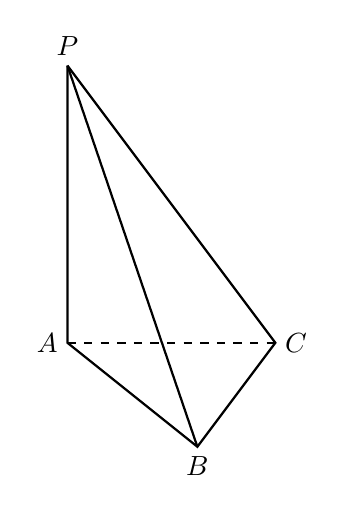
\begin{tikzpicture}[>=stealth, scale=1.1]
  % 顶点坐标
  \coordinate (A) at (0, 0);
  \coordinate (P) at (0, 3.2);
  \coordinate (C) at (2.4, 0);
  \coordinate (B) at (1.5, -1.2);

  % 实线棱
  \draw[thick] (P) -- (A) -- (B) -- (C) -- (P);
  \draw[thick] (P) -- (B);

  % 虚线棱
  \draw[dashed, thick] (A) -- (C);

  % 顶点标签
  \node[above] at (P) {$P$};
  \node[left] at (A) {$A$};
  \node[below] at (B) {$B$};
  \node[right] at (C) {$C$};
\end{tikzpicture}
\end{center}
\nopagebreak[4]
\end{question}
\begin{question}
\gkti{14}在数列 $\{a_n\}$ 中，$a_1 = 1$，$a_2 = 2$，且 $a_{n+2} - a_n = 1 + (-1)^n$ ($n \in \mathbb{N}^*$)，则 $S_{10} = \underline{\hspace{2em}}$．

\end{question}
\begin{question}
\gkti{15}在直角坐标系 $xOy$ 中，已知点 $A(0, 1)$ 和点 $B(-3, 4)$，若点 $C$ 在 $\angle AOB$ 的平分线上且 $|\vec{OC}| = 2$，则 $\vec{OC} = \underline{\hspace{2em}}$．

\end{question}
\begin{question}
\gkti{16}设函数 $f(x) = \ln\dfrac{1+x}{1-x}$，则函数 $g(x) = f\left(\dfrac{x}{2}\right) + f\left(\dfrac{1}{x}\right)$ 的定义域为 $\underline{\hspace{2em}}$．

\Needspace{0.4\textheight}
\end{question}
\begin{question}
\gkti{17}在三角形的每条边上各取三个分点（如图）．以这 $9$ 个分点为顶点可画出若干个三角形，若从中任意抽取一个三角形，则其三个顶点分别落在原三角形的三条不同边上的概率为 $\underline{\hspace{2em}}$．（用数字作答）
\nopagebreak[4]
\begin{center}\begin{tikzpicture}[>=stealth, scale=0.9]
  % 三角形顶点
  \coordinate (A) at (0, 0);
  \coordinate (B) at (4.0, 0);
  \coordinate (C) at (2.0, 3.464);

  % 边
  \draw[thick] (A) -- (B) -- (C) -- cycle;

  % 底边 3 个分点
  \foreach \i in {1, 2, 3} {
    \fill ($ (A) ! \i/4 ! (B) $) circle (1.8pt);
  }

  % 右边 3 个分点
  \foreach \i in {1, 2, 3} {
    \fill ($ (B) ! \i/4 ! (C) $) circle (1.8pt);
  }

  % 左边 3 个分点
  \foreach \i in {1, 2, 3} {
    \fill ($ (C) ! \i/4 ! (A) $) circle (1.8pt);
  }
\end{tikzpicture}
\end{center}
\nopagebreak[4]
\end{question}
\gkpart{三、解答题：本大题共 6 小题，共 72 分．解答应写出文字说明，证明过程或演算步骤．}

\begin{question}
\gkti{18}（本小题满分 12 分）
已知 $\sin\left(\alpha - \dfrac{\pi}{4}\right) = \dfrac{7\sqrt{2}}{10}$，$\cos 2\alpha = \dfrac{7}{25}$，
(1) 求 $\sin\alpha$ 的值；
(2) 求 $\tan\left(\alpha + \dfrac{\pi}{3}\right)$ 的值．

\end{question}
\begin{question}
\gkti{19}（本小题满分 12 分）
若公比为 $c$ 的等比数列 $\{a_n\}$ 的首项 $a_1 = 1$ 且满足 $a_n = \dfrac{a_{n-1} + a_{n-2}}{2}$ ($n = 3, 4, \cdots$)．
(1) 求 $c$ 的值；
(2) 求数列 $\{n a_n\}$ 的前 $n$ 项和 $S_n$．

\Needspace{0.4\textheight}
\end{question}
\begin{question}
\gkti{20}（本小题满分 12 分）
如图，在斜三棱柱 $ABC - A_1B_1C_1$ 中，$\angle A_1AB = \angle A_1AC$，$AB = AC$，$A_1A = A_1B = a$，侧面 $B_1BCC_1$ 与底面 $ABC$ 所成的二面角为 $120^\circ$，$E$、$F$ 分别是棱 $B_1C_1$、$A_1A$ 的中点．
\nopagebreak[4]
\begin{center}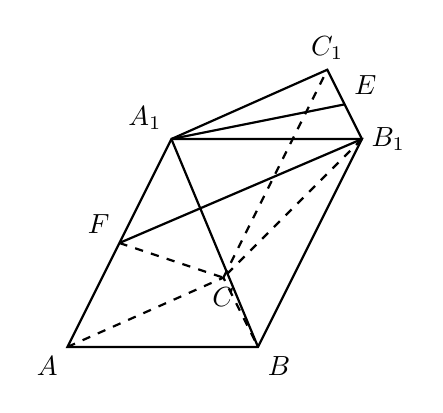
\begin{tikzpicture}[>=stealth, scale=1.1]
  % 底面顶点
  \coordinate (A) at (0, 0);
  \coordinate (B) at (2.2, 0);
  \coordinate (C) at (1.8, 0.8);

  % 侧棱向量: (1.2, 2.4)
  \coordinate (A1) at (1.2, 2.4);
  \coordinate (B1) at (3.4, 2.4);
  \coordinate (C1) at (3.0, 3.2);

  % 中点 F on A1A, E on B1C1
  \coordinate (F) at (0.6, 1.2);
  \coordinate (E) at (3.2, 2.8);

  % 实线棱
  \draw[thick] (A) -- (B) -- (B1) -- (A1) -- cycle;
  \draw[thick] (A1) -- (C1) -- (B1);
  \draw[thick] (A1) -- (B);
  \draw[thick] (A1) -- (E);
  \draw[thick] (B1) -- (F);

  % 虚线棱与辅助线
  \draw[dashed, thick] (A) -- (C) -- (B);
  \draw[dashed, thick] (C) -- (C1);
  \draw[dashed, thick] (F) -- (C);
  \draw[dashed, thick] (B1) -- (C);

  % 顶点标签
  \node[below left] at (A) {$A$};
  \node[below right] at (B) {$B$};
  \node[below] at (C) {$C$};
  \node[above left] at (A1) {$A_1$};
  \node[right] at (B1) {$B_1$};
  \node[above] at (C1) {$C_1$};
  \node[above left] at (F) {$F$};
  \node[above right] at (E) {$E$};
\end{tikzpicture}
\end{center}
\nopagebreak[4]
(1) 求 $A_1A$ 与底面 $ABC$ 所成的角；
(2) 证明 $A_1E \parallel \text{\text{平面} } B_1FC$；
(3) 求经过 $A_1, A, B, C$ 四点的球的体积．

\Needspace{0.4\textheight}
\end{question}
\begin{question}
\gkti{21}（本小题满分 12 分）
某人在一山坡 $P$ 处观看对面山顶上的一座铁塔，如图所示，塔高 $BC = 80$（米），塔所在的山高 $OB = 220$（米），$OA = 200$（米），图中所示的山坡可视为直线 $l$ 且点 $P$ 在直线 $l$ 上，$l$ 与水平地面的夹角为 $\alpha$，$\tan\alpha = \dfrac{1}{2}$．试问此人距水平地面多高时，观看塔的视角 $\angle BPC$ 最大？（不计此人的身高）
\nopagebreak[4]
\begin{center}\begin{tikzpicture}[>=stealth, scale=0.85]
  % 基准坐标
  \coordinate (O) at (0, 0);
  \coordinate (A) at (2.0, 0);
  \coordinate (B) at (0, 2.6);
  \coordinate (C) at (0, 3.5);
  \coordinate (P) at (3.8, 0.9);

  % 水平地面虚线
  \draw[dashed, thick] (O) -- (5.6, 0) node[right] {水平地面};
  % 山高 OB 虚线
  \draw[dashed, thick] (O) -- (B);

  % 铁塔 BC
  \draw[thick] (-0.15, 2.6) -- (0.15, 2.6) -- (0, 3.5) -- cycle;

  % 山坡 l 射线
  \draw[thick] (A) -- (5.4, 1.7) node[above right] {$l$ (山坡)};

  % 视线 PB, PC
  \draw[thick] (P) -- (B);
  \draw[thick] (P) -- (C);

  % 坡角 alpha 标注
  \draw (2.7, 0) arc (0:26.565:0.7);
  \node at (2.9, 0.2) {$\alpha$};

  % 顶点标签
  \node[below left] at (O) {$O$};
  \node[left] at (B) {$B$};
  \node[above] at (C) {$C$};
  \node[below] at (A) {$A$};
  \node[below right] at (P) {$P$};
\end{tikzpicture}
\end{center}
\nopagebreak[4]
\end{question}
\begin{question}
\gkti{22}（本小题满分 12 分）
已知 $m \in \mathbb{R}$，设 $P$：$x_1$ 和 $x_2$ 是方程 $x^2 - ax - 2 = 0$ 的两个实根，不等式 $|m^2 - 5m - 3| \geqslant |x_1 - x_2|$ 对任意实数 $a \in [-1, 1]$ 恒成立；$Q$：函数 $f(x) = x^3 + mx^2 + \left(m + \dfrac{4}{3}\right)x + 6$ 在 $(-\infty, +\infty)$ 上有极值．求使 $P$ 正确且 $Q$ 正确的 $m$ 的取值范围．

\end{question}
\begin{question}
\gkti{23}（本小题满分 12 分）
抛物线 $C$ 的方程为 $y = ax^2$ ($a < 0$)，过抛物线 $C$ 上一点 $P(x_0, y_0)$ ($x_0 \neq 0$) 作斜率为 $k_1, k_2$ 的两条直线分别交抛物线 $C$ 于 $A(x_1, y_1)$、$B(x_2, y_2)$ 两点（$P, A, B$ 三点互不相同），且满足 $k_2 + \lambda k_1 = 0$ ($\lambda \neq 0, \lambda \neq -1$)．
(1) 求抛物线 $C$ 的焦点坐标和准线方程；
(2) 设直线 $AB$ 上一点 $M$，满足 $\vec{BM} = \lambda \vec{MA}$，证明线段 $PM$ 的中点在 $y$ 轴上；
(3) 当 $\lambda = 1$ 时，若点 $P$ 的坐标为 $(1, -1)$，求 $\angle PAB$ 为钝角时点 $A$ 的纵坐标 $y_1$ 的取值范围．

\end{question}